%%%%%%%%%%%%%%%%%%%%%%%%%%%%%%%%%%%%%%%%%
% Intermediate report
% Version 1.0 (10/16/13)
%
% This template has been downloaded from:
% http://www.LaTeXTemplates.com
%
% Original Authors:
% Darren Chu
% Todd Detweiler
% Cody Kagawa
% Lauren Swanson
% Dogni Wang
%
%%%%%%%%%%%%%%%%%%%%%%%%%%%%%%%%%%%%%%%%%

%----------------------------------------------------------------------------------------
%	PACKAGES AND OTHER DOCUMENT CONFIGURATIONS
%----------------------------------------------------------------------------------------

\documentclass[a4paper, 11pt]{article} % Font size (can be 10pt, 11pt or 12pt) and paper size (remove a4paper for US letter paper)

\usepackage[protrusion=true,expansion=true]{microtype} % Better typography
\usepackage{graphicx} % Required for including pictures
\usepackage{wrapfig} % Allows in-line images
\usepackage{pdfpages}

\usepackage{mathpazo} % Use the Palatino font
\usepackage[T1]{fontenc} % Required for accented characters
\linespread{1.05} % Change line spacing here, Palatino benefits from a slight increase by default

\DeclareGraphicsExtensions{.pdf,.png,.jpg}


\makeatletter
\renewcommand\@biblabel[1]{\textbf{#1.}} % Change the square brackets for each bibliography item from '[1]' to '1.'
\renewcommand{\@listI}{\itemsep=0pt} % Reduce the space between items in the itemize and enumerate environments and the bibliography

\renewcommand{\maketitle}{ % Customize the title - do not edit title and author name here, see the TITLE block below
\begin{flushright} % Right align
{\LARGE\@title} % Increase the font size of the title

\vspace{50pt} % Some vertical space between the title and author name

{\large\@author} % Author name
\\\@date % Date

\vspace{40pt} % Some vertical space between the author block and abstract
\end{flushright}
}

%----------------------------------------------------------------------------------------
%	TITLE
%----------------------------------------------------------------------------------------

\title{\textbf{Intermediate Report for Object Creator Team}} 

\author{\textsc{Darren Chu\\Todd Detweiler\\Cody Kagawa\\Lauren Swanson\\Dongni Wang} % Author
\\{\textit{University of Puget Sound}}} % Institution

\date{\today} % Date

%----------------------------------------------------------------------------------------

\begin{document}

\maketitle % Print the title section

%----------------------------------------------------------------------------------------
%	ESSAY BODY
%----------------------------------------------------------------------------------------

\section*{Design Specification}

Our module will have four major components including a way to create an image, edit an image, save image, and a way to export the object as a JSON object. The Image Creation class will include functions to draw on a canvas, import an image, or use primitive shapes to construct each individual object. Image Creation will require a canvas, which will be provided by the Javascript Library. The canvas will report the coordinates of the object to facilitate conversion into .png format. Next, the Image Editing class will allow the user to manipulate the size and color of the object, while also providing access to an undo button. The functions of the Image Editing class will be accessible to the user through a toolbar type user interface. Thirdly, there will be a Save Image class which allows users to save pieces of their full object as .png files. And finally, Export Object will be a class which is called upon exiting the canvas and will send the group of saved pieces to the Sharing Framework as a JSON object.

The Image Creation window, alongside our canvas window, will prompt the user begin drawing a part. This prompt will acknowledge that the user is drawing a part of the character, which will be saved as a unique object. The user will be responsible for designating a name for the object, e.g. head.png, to identify it for use in other modules. If the user chooses to draw their character, they will do so by drawing, naming, and saving each part individually. The Save Image class will save each piece as a .png file in a position in an array. When the user is finished saving each piece of their object, they will exit out of the Object creation window. The act of exiting will call our Export Object class, which will export the array of saved .png images to the Sharing Framework as a JSON object(s). Once it is on the sharing framework, the object and its pieces can be accessed and manipulated by other modules. Below, full UML class diagrams of these three major components and their functions are shown.

%------------------------------------------------

\section*{Design Rationale}

To create our model, we will be implementing an Abstract Factory software design pattern. We have chosen this design pattern because our module is based on creating objects but will create those objects in different fashions. The user can either import an image, draw, or build a character out of primitive geometric shapes. All three of these classes will accomplish the same goal of creating an image that will later be used as an object throughout the application. Our other classes will provide the functions of editing and saving this object. An Abstract Factory design pattern is defined as one which groups individual factories that have a common theme. Because all of our classes deal with the larger picture of creating an image and forming an object but do it in different forms, we believe that an Abstract Factory design pattern best fulfills the architecture we have laid out.

%------------------------------------------------

\section*{Design Architecture UML Diagram}
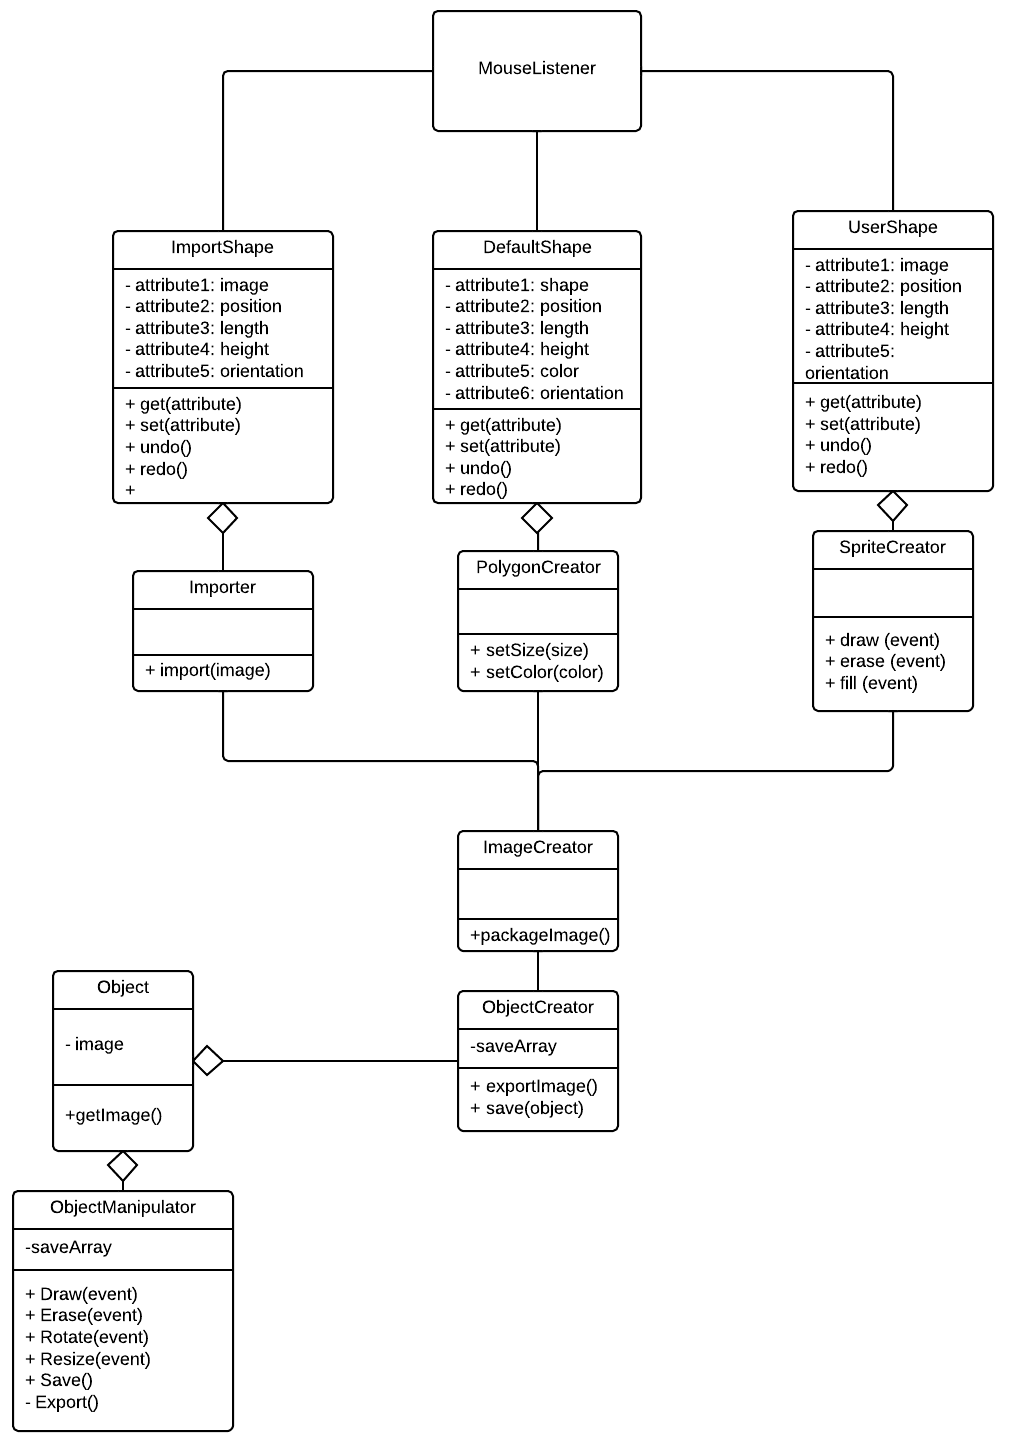
\includegraphics[scale=0.52]{ClassDiagramObjectModule}\\
Internal Diagram: The internal UML diagram shows the basic layout of our module. Most of the module is dedicated to object creation, which will be handled differently depending on the source of the image. The module should take mouse and text commands to arrange various shapes.  Images will be composed of various shapes, which will be packed into objects that can be saved and transported. These objects will also be accessible to the object manipulator, which will handle changes to existing objects.\\
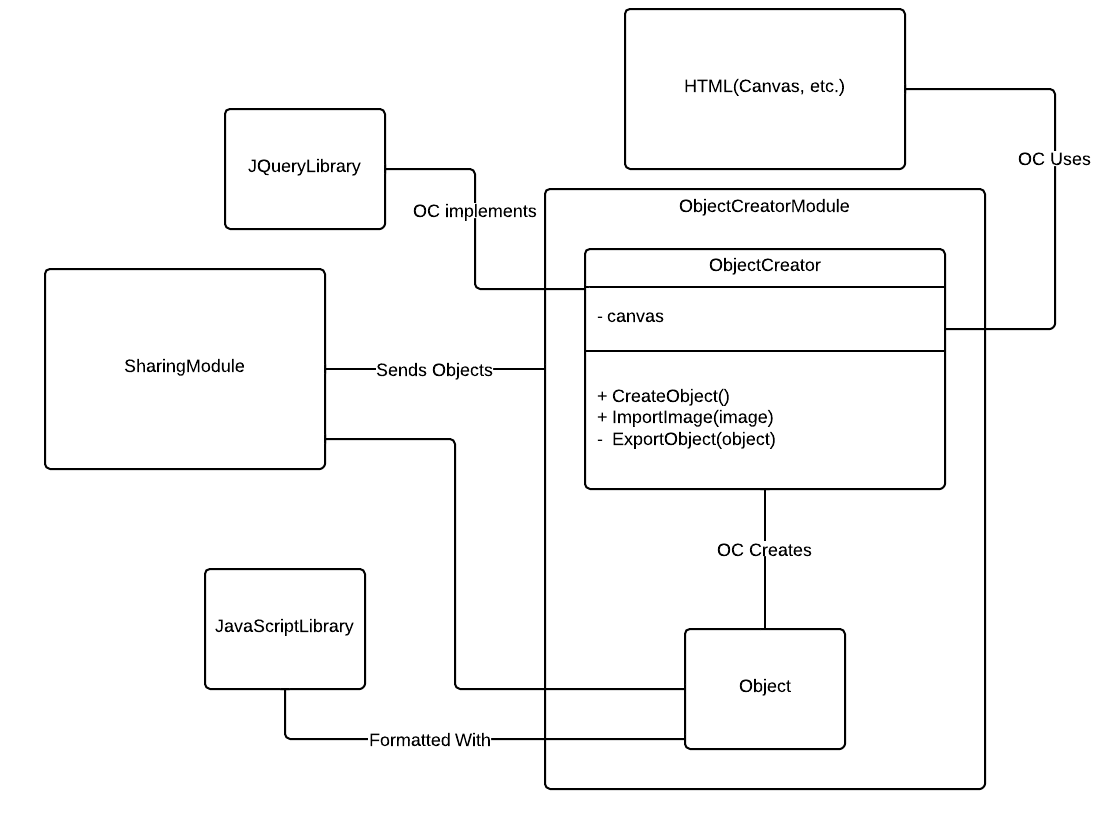
\includegraphics[scale=0.52]{ExternalFlowChart}\\
External Diagram: The external UML diagram lays out our module's interaction with other systems and modules. The objects the module creates will be passed to and from the sharing module whenever an object is created or altered. The module itself will create its own instance of an HTML canvas which we will manipulate using Javascript and JQuery methods.

%------------------------------------------------

\section*{Project Status}

The current state of our module is at the end of the design and planning phase. We have determined the structure of our module and how the user will interact with our functions. We have also determined how our module will interact with other modules of the application. We have established that our module will be exporting JSON array objects filled with .png files to the Sharing Framework. Before our first implementation stage, we will create four different functions. The following team members will be responsible for their listed implementations. Todd will be responsible for a general layout of our canvas, Cody for a free drawing function, Lauren for a saving and exporting function, and Dongni and Darren for the geometric drawing function. All members will collaborate on each part and provide assistance where needed. The timeline of our completion and implementation checkpoints can be seen on the Gantt timeline below.

%------------------------------------------------

\section*{Project Timeline}

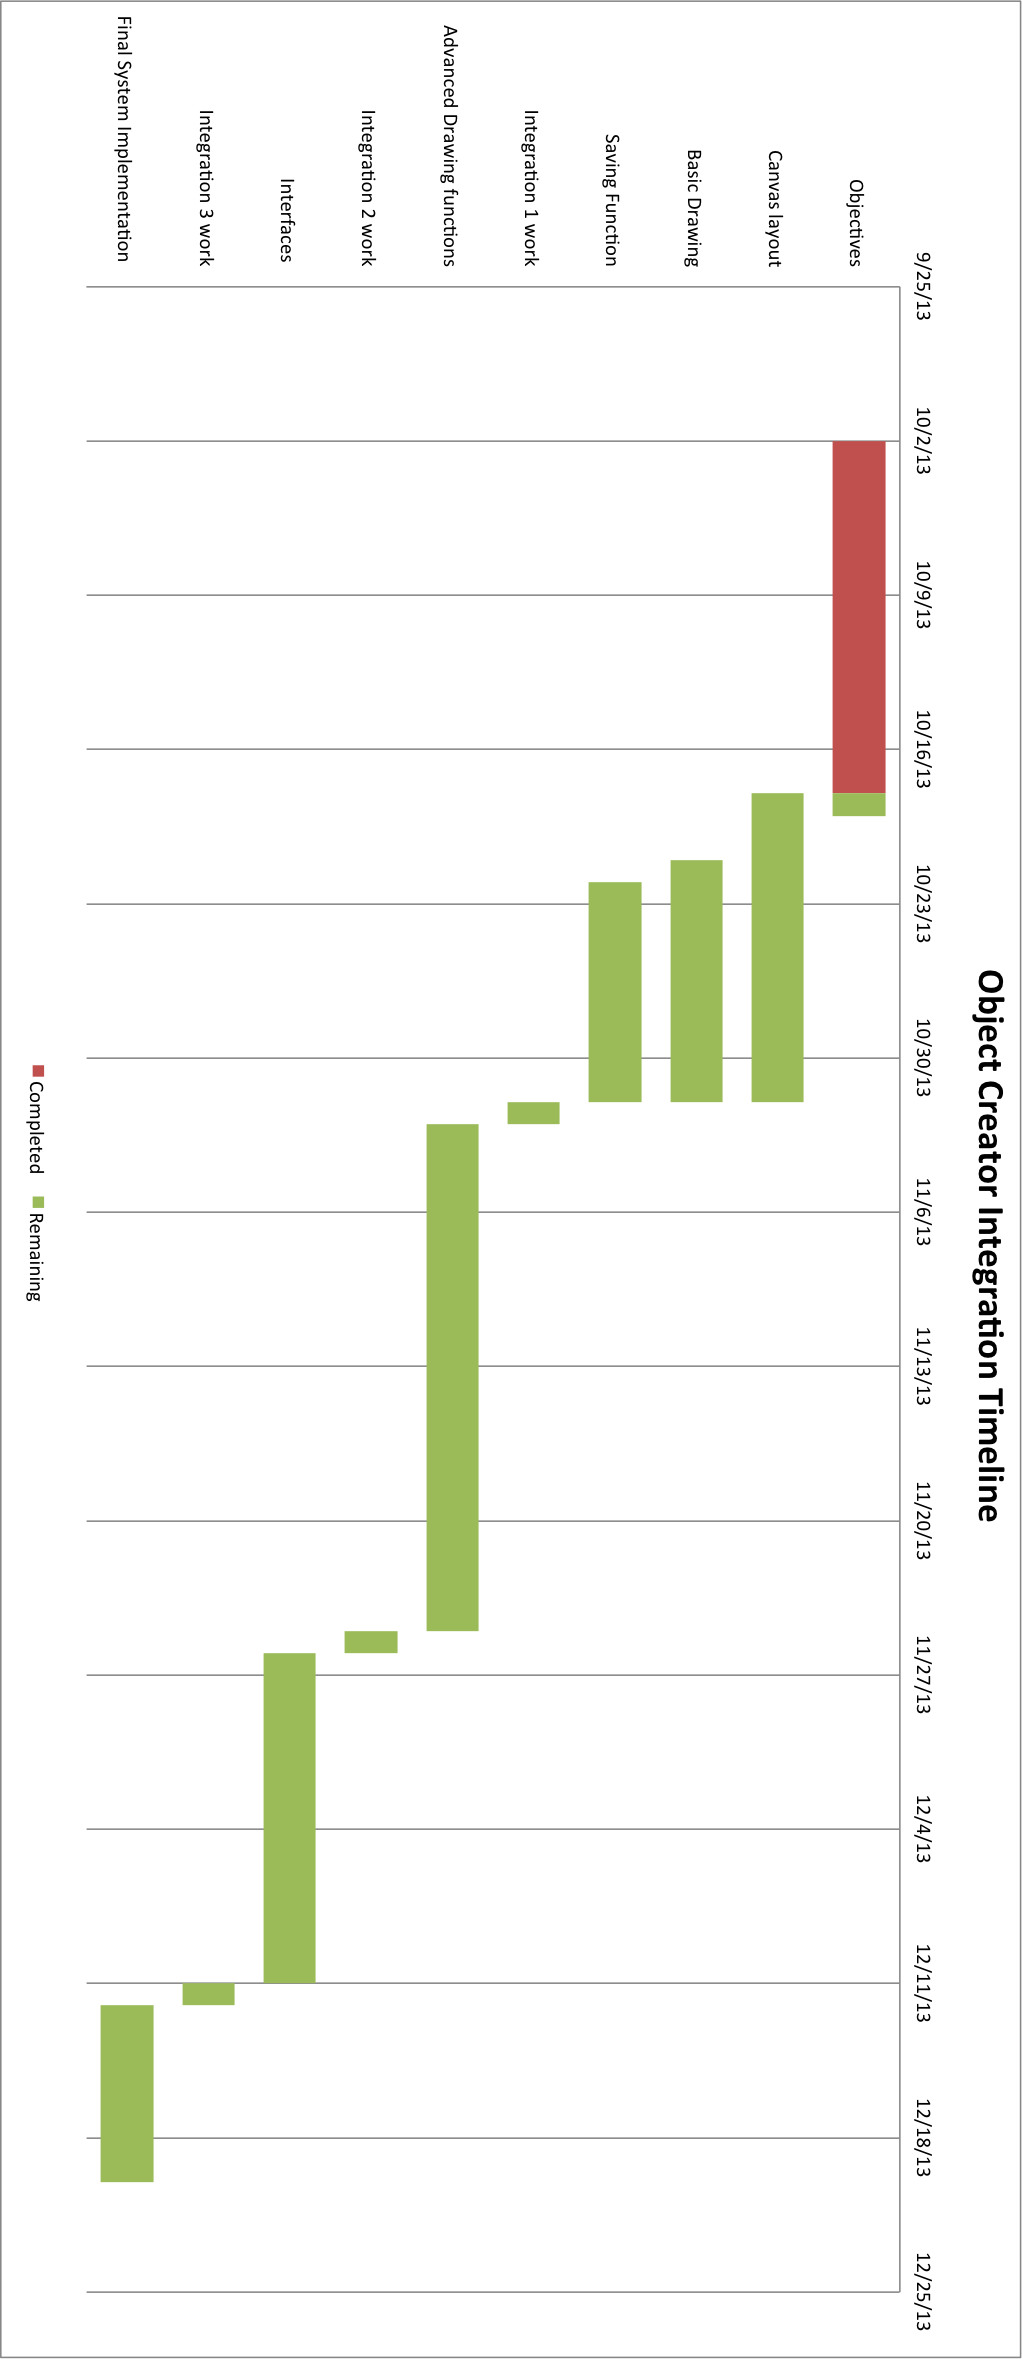
\includegraphics[scale=0.35]{Timeline}\\

First of all, Todd will implement the canvas where all the drawing will place. Once we have the canvas working, we will work on implementing the basic drawing functions and saving function. The basic drawing functions are free-drawing function (Users will be able to draw dots/free-lines using mouse --Cody) and geometric-drawing function (Users will be able to draw basic geometric shapes like triangles/rectangles/circles, etc --Dongni \& Darren). At the same time, saving function (save the canvas as JSON object-- .png and pass it to sharing framework) will be implemented by Lauren. Each function will be tested separately and ready for the first integration.

Integration 1 work:
During this time,  we will put  the basic drawing function and saving functions together, test and adjust each function to make sure they will still be functional together. Also we will communicate with other teams to ensure that each module runs within the same system as the others.

Integration 2 work: our module should be communicating with every other module. The user should be able to draw objects  and see its result used in another. The work for this section will be divided up after we get far enough in integration 1 that we can assess who is best suited to these tasks.

Integration 3 work: the entire system should be integrated to work smoothly together. We should be working on ease of use and efficiency so work will be divided as necessary.

%------------------------------------------------

\section*{Insight on Development Process}

Our process thus far has involved assembling ideas and information on Google Drive, then meeting in person to discuss. There have been some problems with Github and Latex as a result but it has improved our decision-making process as well as our collective understanding of our goals and responsibilities. We experienced some issues in particular with overwriting work on Github and as a result have become more aware of the need to thoroughly proofread our work. Moving forward, we are looking to work out more time to meet and discuss the code as a group. We have also realized how important our module is to a number of other groups and are planning to maintain communication with other groups.We have formed solid plans for the future and have laid out the groundwork for the future implementation of our module. 

%------------------------------------------------

\section*{User Interface Interaction and Mockup}

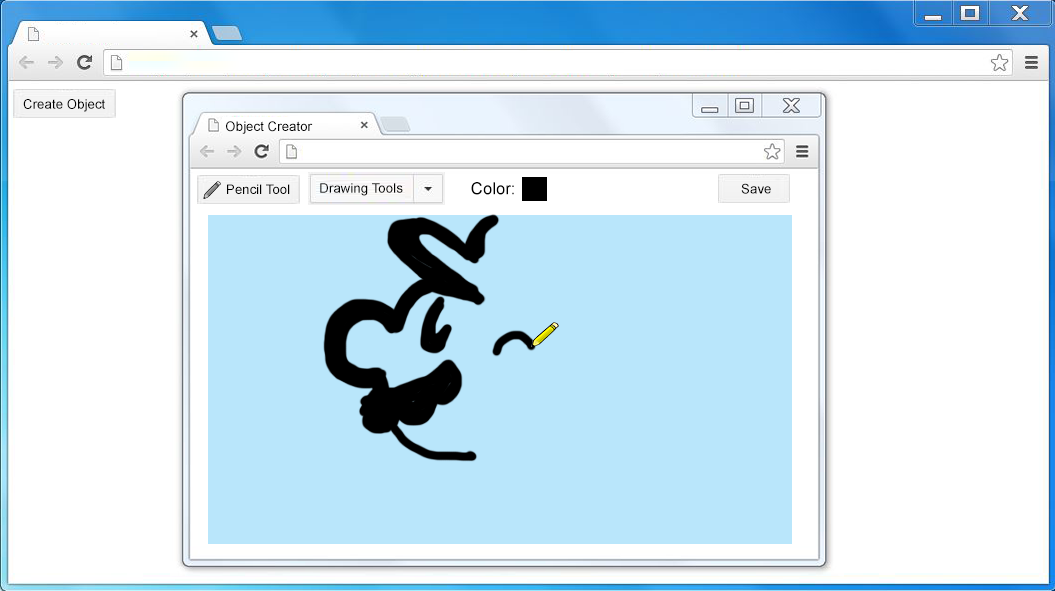
\includegraphics[scale=0.58]{Mockup}\\

The Object Creator should generate its own window as part of the interface and should invalidate any commands to the canvas until the object creator is closed. The interface will allow for interaction primarily through use of assigned buttons and reading mouse commands within the canvas bounds, with a few drag and drop methods. Drawing functions will be separated from geometry tools and closing the window should send any saved objects to permanent storage. Geometric tools will require that the user specify an action prior to each command, whereas drawing tools will allow for sequences of commands, or continuous inputs depending on the tool selected. Certain geometric tools will utilize text boxes to designate height and width, as well as initial saves to specify object names.

%----------------------------------------------------------------------------------------
%	BIBLIOGRAPHY
%----------------------------------------------------------------------------------------

\bibliographystyle{unsrt}

\section*{Bibliography}

Diaz, Nicholas. "Latex Templates.". Latex Templates, 16 03 2013. Web. 16 Oct 2013. <http://www.latextemplates.com/template/thin-sectioned-essay>.

%----------------------------------------------------------------------------------------

\end{document}